\section{Geoscape}

\subsection{Worldmap - an overview} 
Welcome to Geoscape! As said before UFO:AI distincts between two major aspects of the game -- macromanagement and tactical combat. To put it simply, one could say: Combat is where you earn the bucks (and the honour, of course), Geoscape is where you spend them.

Geoscape itself basically consists of two screens. The first one is the world map, which is the first screen you will see right after starting a new campaign. It is used to get the bigger picture of world events as well as coordinating combat missions and intercepting enemy UFOs. The other screen is the base overview, where you improve infrastructure and implement decisions about equipment, research and production. In the following sections we will take a closer look at both of these screens.

The following screenshot shows the uses to which we can put the world map. Observe that it is divided into day and night zones, which influences any combat missions you get into (the day/night borderline changes its shape according to the seasons as the relation earth to sun changes).\\

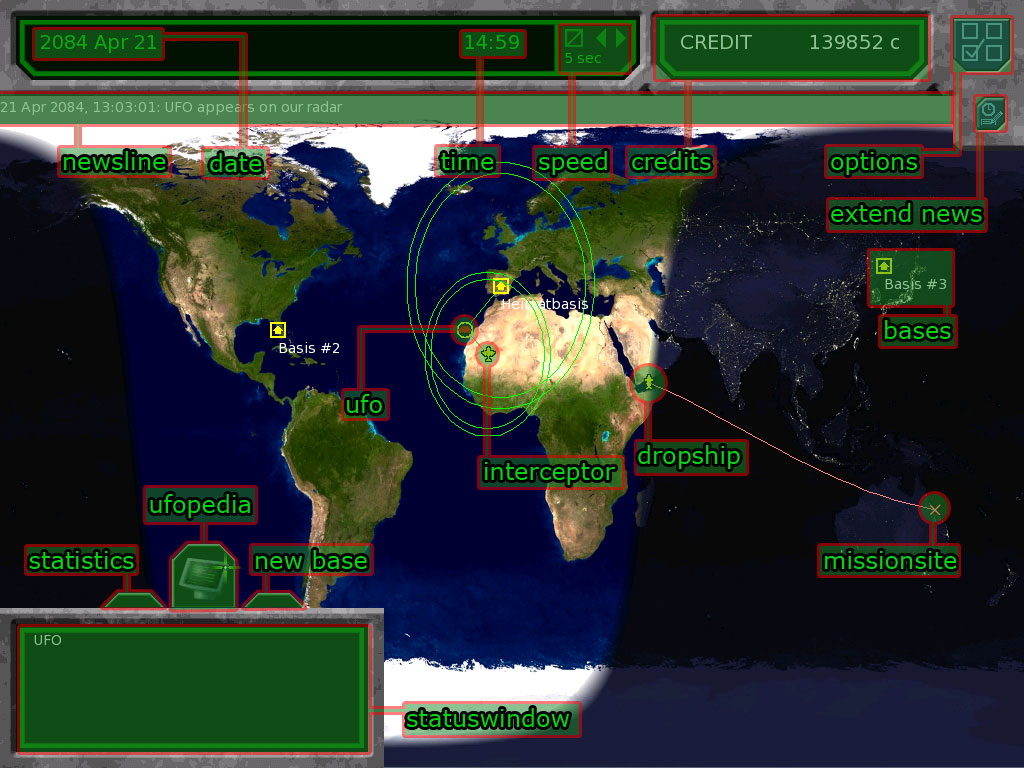
\includegraphics[width=\textwidth]{images/geoscape_final.jpg}

\newpage

\subsubsection{Status Window}
Here some general information(e.g. stats, descriptions) will show up, depending on the context. More detail on each piece of information is given in subsequent sections.
\subsubsection{Statistics}
If you hover over those registers three different buttons will show up. The leftmost leads to some more detailed statistics about your attempt to save the world. In addition to more general information (like missions won/lost etc.) you can also find out about the attitude of all the UN countries paying you. You should be aware that if you fail to protect particular countries from alien invasions (maybe because your infrastructure is not well established in that region) they will cut your resources -- both financial and potential employees.
\subsubsection{Ufopedia}
The middle button is the Ufopedia, a comprehensive collection of useful information about items, technologies, damage types and so on. As your research proceeds Ufopedia grows as well, so make sure you check out the latest information on your enemies every now and then.
\subsubsection{New base}
The rightmost button gives you the chance to establish a new base anywhere on the map, provided it's on land. A new base, once you have built new structures, can give additional radar range, research and production capacities as well as new hangars for your aircraft.  New bases are completely equal to your first in all ways.
\subsubsection{Date}
Gives you the current date, so you know when it's close to pay day. You should also keep an eye on the date, because while you (in principle) have unlimited time to play the game, the aliens get stronger and better equipped as the game proceeds. It is in humanity's best interest if you can catch up with them sooner than later in order to save your beloved homeworld.
\subsubsection{Time and Game Speed}
This is where you can adjust the gamespeed from 5secs (which is in fact pausing the game) all the way through to 1 day steps. Whatever this is set to, while you are in combat time is stopped and it will be all the same when you return from battle.  The game will also automatically pause for certain events like UFO spottings and landings.
\subsubsection{Credits}
Never forget that you can't spend what you don't have.
\subsubsection{Options}
Gets you to the Options-menu where you can load and save your game as well as start a new one.
Through ``exit'' you reach the main menu where you can change game settings and continue your current game (via Single Player $\rightarrow$ Continue)
\subsubsection{News and extended news}
The permanent news line in the upper left always represents the latest news (such as promotions / cashflow / attacks / UFO-sightings) while the extended news button pops up a list of the last 20 new lines. So whenever you notice news, make sure to check the button as well so you don't miss anything. 
\subsubsection{Bases}
The yellow houses represent your bases. Circles around them (popping up later in the game) represent the range of their radars. If you want to ``enter'' a base, just click on its symbol.
\subsubsection{Your dropship}
This is the one that gets your squad to action. Clicking on it once brings up some general data about your ship, like fuel, speed, status and number of assigned soldiers. A second click while it's selected opens a submenu where you may give/change orders, such as sending it back home.
\subsubsection{Your interceptors}
The job of those fast ships is to shoot enemy UFOs down. If your interceptor catches up with a UFA, the dogfight is calculated based on the equipment of both ships; the results are shown on screen. A single click selects the interceptor, while a click on the map will order it to move it there. A second click while the ship is selected brings up a window where you might give it more advanced orders.
\subsubsection{Upcoming missions}
This is where the action waits. Selecting a mission will give you a short description on the status screen while a second one allows you to select a ship to bring in the troops you want.